\section{The Research Object Model}
\label{sec:model}

The Wf4Ever Research Object model defines vocabularies that describe Workflow-centric Research Objects within Wf4Ever. A complete, functional RO based ecosystem also requires a number of different services for creation, storage, manipulation, recommendation, visualisation etc. of Research Objects. These services are not considered as part of the model (although implemented services are described in this deliverable in Sections~\ref{sec:rosrs} and \ref{sec:manager}). Nor does the core model describe the evolution of Research Objects (ROs) -- this is discussed in D3.2v1~\cite{D3.2v1}.

Narrative text describing the model is published online\footnote{\url{http://wf4ever.github.com/ro/}} and the ontologies themselves also available\footnote{\url{https://github.com/wf4ever/ro/}}. We will not reproduce all this narrative text here, but provide an overview of the model and rationale.

A simple schematic of an RO is shown in Figure~\ref{fig:ro}. The RO contains a workflow, input data and results along with a paper that presents the results and links to the investigators responsible. Annotations on each of the resources (and on the RO itself) provide additional information and characterise, e.g. the provenance of the results (the results were obtained by executing the workflow on the input data). 

\begin{figure}[ht]
  \centering
  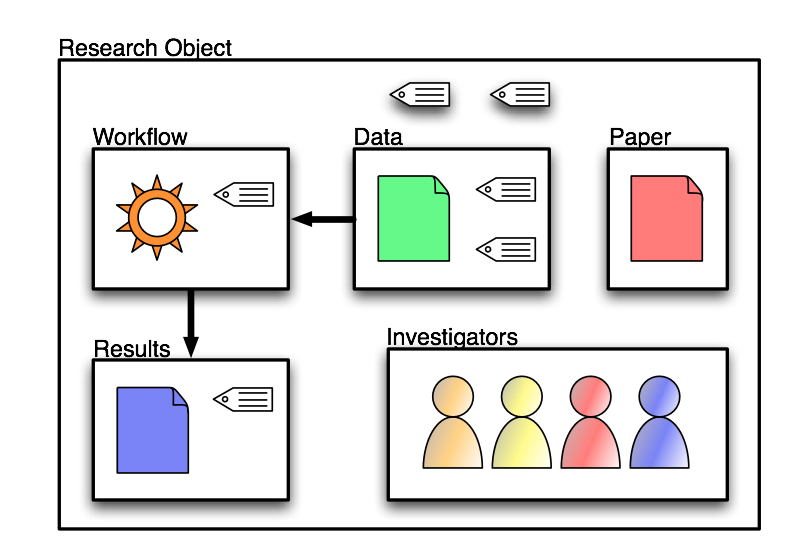
\includegraphics[width=0.4\textwidth]{Figures/RO-cartoon}
  \caption{RO Schematic}
  \label{fig:ro}
\end{figure}
 Research Objects play multiple roles. In the first case, they are \emph{technical} objects. They provide access to the resources that are needed to support execution of investigations and record the provenance traces of those executions. They encapsulate dependencies between resources and maintain versioning information about the lineage and evolution of those resources.

At the same time, they are \emph{social} objects. They encapsulate reusable protocols and know-how. They record best practices and support reproducibility. They are citable artifacts that can be referred to and quoted. They record and represent information about the people involved in investigations -- those who create, use, extend and curate the objects.

These roles bring requirements on the representation structure and vocabularies used to describe Research Objects. The specification of the RO model focuses on the technical aspects. It describes the core Wf4Ever Research Object vocabularies that provide container structures and vocabulary for describing workflow objects. Additional vocabularies covering evolution, lifecycle, versioning and other social aspects will be covered elsewhere.

ROs allow for the aggregation of resources along with annotations on
those resources concerning their provenance, use, characteristics
etc. Aggregation is supported through the use of the OAI-ORE
vocabulary\footnote{OAI-ORE is not a ratified standard
  produced by a body such as the W3C or IETF, but it is becoming
  widely used as a vocabulary for aggregation.} and annotation is
supported through the use of the Annotation Ontology\footnote{Again,
  AO is not as yet a standardised vocabulary, but a W3C community
  group has been set up to oversee the drafting of a specification: \url{http://www.w3.org/community/openannotation/}}. Re-use of these existing vocabulary will facilitate third party tools in understanding and processing Research Objects described using the model. 


Finally, the RO Model provides a number of basic ontologies that are used within this aggregation/annotation framework to describe specifics of the Workflow-centric Research Objects. These are:

\begin{description}
\item[ro] Provides basic structure for the description of aggregated
  resources and the annotations that are made on those resources.
\item[wfdesc] A vocabulary for the description of workflows. This
  provides an abstraction that can be mapped to different particular
  workflow systems. The ontology is intended as an upport ontology for more specific workflow definitions, and as a way to express abstract workflows, which could either be hand-crafted by users, or extracted from workflow definitions, for example Taverna's \texttt{t2flow} or Scufl2 formats. A prototype service that transforms workflows into Research Objects, using the wfdesc ontologies has been developed (See~\cite{D1.4v1}). 
\item[wfprov] A vocabulary for the description of provenance
  information. This provides an abstraction that can be mapped to
  different provenance vocabularies, for example PROV-O\footnote{\url{http://www.w3.org/TR/prov-o/}} as developed by the W3C Provenance Working Group.
\end{description}

